% begin module differentials-intro
\begin{frame}
\frametitle{ %(3.9)
Linear Approximations and Differentials}
\begin{itemize}
\item Main idea: A curve is very close to its tangent line at the point of tangency.
\item We can use the tangent line at $(a,f(a))$ as an approximation to the curve $y = f(x)$.
\item This approximation works well as long as $x$ is near $a$.
\end{itemize}
%\begin{center}
\psset{xunit=1cm, yunit=1cm}
\begin{pspicture}(-0.5,-0.5)(5.1,2.6)
\tiny
\psframe*[linecolor=white](-0.5,-0.5)(5.1,2.6)
\psaxes[ticks=none, labels=none]{<->}(0,0)(-0.5,-0.5)(5,2.5)
\rput(4,1.5){$y=L(x)$}
\rput (4,2.5 ){$y=f(x)$}
%Function formula: (3/5+1/5 (x))^{2}
\psplot[linecolor=red, plotpoints=1000]{0}{5}{x 0.2 mul 0.6 add 2 exp }
%Function formula: 1/5+2/5 (x)
\psplot[linecolor=blue, plotpoints=1000]{0}{5}{x 0.4 mul 0.2 add } \rput[b](2, 1.2){$(a, f(a))$}
\fcFullDotBlack{2}{1}
\end{pspicture}
%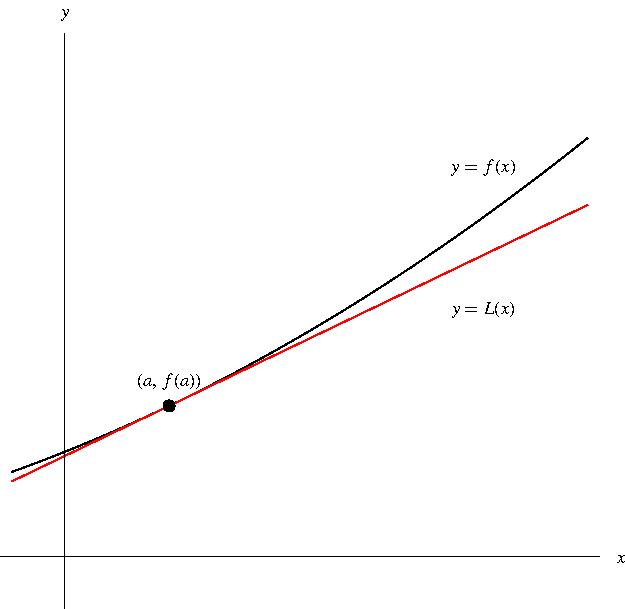
\includegraphics[height=4cm]{differentials/pictures/03-09-linapprox.pdf}%
%\end{center}
\end{frame}
% end module differentials-intro
